\documentclass[letterpaper,11pt]{article}

\usepackage{amsmath}
\usepackage{amssymb}
\usepackage[hmargin=1.25in,vmargin=1in]{geometry}
\usepackage{booktabs}
\usepackage{graphicx}
\usepackage{hyperref}
\usepackage{lmodern}
\usepackage{microtype}
\usepackage{pdflscape}
\usepackage{subcaption}

\title{Coursework 5: STAT 570}
\author{Philip Pham}
\date{\today}

\begin{document}
\maketitle

\begin{enumerate}
\item Consider the data given in Table \ref{tab:p1_data}, which are a simplified
  version of those reported in Breslow and Day (1980). These data arose from a
  case-control study that was carried out to investigate the relationship
  between esophageal cancer and various risk factors. Disease status is denoted
  $Y$ with $Y = 0$ and $Y = 1$ corresponding to without/with disease and alcohol
  consumption is represented by $X$ with $X = 0$ and $X = 1$ denoting less than
  80g and greater than or equal to 80g on average per day. Let the probabilities
  of high alcohol consumption in the cases and controls be denoted

  \begin{equation}
    p_1 = \mathbb{P}\left(X = 1 \mid Y = 1\right)~\text{and}~
    p_2 = \mathbb{P}\left(X = 1 \mid Y = 0\right),
    \label{eqn:p1_pi_definition}
  \end{equation}
  respectively. Further, let $X_1$ be the number exposed from $n_1$ cases and
  $X_2$ be the number exposed from $n_2$ controls. Suppose
  $X_i \mid p_i \sim \operatorname{Binomial}(n_i,p_i)$ in the case ($i = 1$) and
  control ($i = 2$) groups.
  
  \begin{table}
    \centering
    \begin{tabular}{l|cc|c}
      & $X = 0$ & $X = 1$ & \\
      \hline
      $Y = 1$ & 104 & 96 & 200 \\
      $Y = 0$ & 666 & 109 & 775 \\
    \end{tabular}
    \caption{Case-control data: $Y = 1$ corresponds to the event of esophageal
      cancer, and $X = 1$ exposure to greater than 80g of alcohol per day. There
      are 200 cases and 775 controls.}
    \label{tab:p1_data}
  \end{table}

  \begin{enumerate}
  \item Of particular interest in studies such as this is the odds ratio defined
    by
    \begin{equation}
      \theta = \frac{\mathbb{P}\left(Y = 1 \mid X = 1\right)/\mathbb{P}\left(Y = 0 \mid X = 1\right)}
      {\mathbb{P}\left(Y = 1 \mid X = 0\right)/\mathbb{P}\left(Y = 0 \mid X = 0\right)}.
      \label{eqn:p1_odds_ratio}
    \end{equation}

    Show that the odds ratio is equal to
    \begin{equation}
      \theta
      = \frac{\mathbb{P}\left(X = 1 \mid Y = 1\right)/\mathbb{P}\left(X = 0 \mid Y = 1\right)}
      {\mathbb{P}\left(X = 1 \mid Y = 0\right)/\mathbb{P}\left(X = 0 \mid Y = 0\right)}
      = \frac{p_1/(1 - p_1)}{p_2/(1-p_2)}.
      \label{eqn:p1_odds_ratio_solution}
    \end{equation}

    \begin{description}
    \item[Solution:] We have that
      \begin{equation}
        \mathbb{P}\left(Y = y \mid X = x\right)
        = \frac{\mathbb{P}\left(X = x \mid Y = y\right)\mathbb{P}\left(Y = y\right)}{\mathbb{P}\left(
            X = x
          \right)}
        \label{eqn:p1_bayes_rule}
      \end{equation}
      by Bayes' rule. Applying Equation \ref{eqn:p1_bayes_rule} to Equation
      \ref{eqn:p1_odds_ratio}, we get
      \begin{equation}
        \theta = \frac{
          \left[
            \mathbb{P}\left(X = 1 \mid Y = 1\right)\mathbb{P}\left(Y = 1\right)
          \right]/\left[
            \mathbb{P}\left(X = 0 \mid Y = 1\right)\mathbb{P}\left(Y = 0\right)
          \right]}{
          \left[
            \mathbb{P}\left(X = 0 \mid Y = 1\right)\mathbb{P}\left(Y = 1\right)
          \right]/\left[
            \mathbb{P}\left(X = 0 \mid Y = 0\right)\mathbb{P}\left(Y = 0\right)
          \right]}.
      \end{equation}
      The $\mathbb{P}\left(Y = y\right)$ factors cancel and we obtain the first
      part of Equation \ref{eqn:p1_odds_ratio_solution}. Using Equation
      \ref{eqn:p1_pi_definition}, we substitute to obtain the second part of
      Equation \ref{eqn:p1_odds_ratio_solution}.
    \end{description}
  \item Obtain the MLE and a 90\% confidence interval for $\theta$, for the data
    of Table \ref{tab:p1_data}.

    \begin{description}
    \item[Solution:]
      The likelihood and log-likelihood functions are
      \begin{align}
        L\left(p_1,p_2\right)
        &= {n_1 \choose x_1}p_1^{x_1}\left(1 - p_1\right)^{n_1 - x_1} +
          {n_2 \choose x_2}p_2^{x_2}\left(1 - p_2\right)^{n_2 - x_2}
          \label{eqn:p1_likelihood}\\
        l\left(p_1,p_2\right)
        &= \log L\left(p_1,p_2\right) \nonumber\\
        &= \sum_{i=1}^2\left[
          \log {n_i \choose x_i} + x_i \log p_i + \left(n_i - x_i\right)\log\left(1 - p_i\right)
          \right],
        \nonumber
      \end{align}
      so the score function is
      \begin{equation}
        S\left(p_1,p_2\right)
        = \nabla \log L\left(p_1,p_2\right)
        = \begin{pmatrix}
          \frac{x_1 - n_1p_1}{p_1\left(1 - p_1\right)} \\
          \frac{x_2 - n_2p_2}{p_2\left(1 - p_2\right)}.
        \end{pmatrix}
        \label{eqn:p1_score}
      \end{equation}
      
      Thus, the Fisher information is
      \begin{equation}
        I\left(p_1,p_2\right) = \mathbb{E}\left[
          S\left(p_1,p_2\right)S\left(p_1,p_2\right)^\intercal
        \right]= \begin{pmatrix}
          \frac{n_1}{p_1\left(1 - p_1\right)} & 0 \\
          0 & \frac{n_2}{p_2\left(1 - p_2\right)}
        \end{pmatrix}.
        \label{eqn:p1_fisher_information}
      \end{equation}

      From Equation \ref{eqn:p1_score}, we can solve
      $S\left(\hat{p}_1,\hat{p}_2\right) = \mathbf{0}$ to get the MLEs
      $\hat{p}_1 = x_1/n_1$ and $\hat{p}_2 = x_2/n_2$. Since the MLE is
      invariant to reparameterization, we have the MLE for $\theta$:
      \begin{equation}
        \boxed{\hat{\theta} = \frac{\hat{p}_1/\left(1 - \hat{p}_1\right)}{\hat{p}_2/\left(1 - \hat{p}_2\right)} = \frac{1992}{1417} \approx 5.640.}
        \label{eqn:p1_theta_mle}
      \end{equation}

      We estimate the confidence interval for $\log\hat{\theta}$ which works
      since $\log$ is a monotonic transform. Using the delta method and Equation
      \ref{eqn:p1_fisher_information}, we have that
      \begin{align}
        \operatorname{Var}\left(
        \log\hat{\theta}\right)
        &\approx \left(\nabla \log\hat{\theta}\right)^\intercal
        \left(I\left(\hat{p}_1,\hat{p}_2\right)\right)^{-1}
          \left(\nabla \log\hat{\theta}\right) \nonumber\\
        &=
          \begin{pmatrix}
            \frac{1}{\hat{p}_1\left(1 - \hat{p}_1\right)} &
            \frac{1}{\hat{p}_2\left(1 - \hat{p}_2\right)}
          \end{pmatrix}
          \begin{pmatrix}
            \frac{\hat{p}_1\left(1 - \hat{p}_1\right)}{n_1} & 0 \\
            0 & \frac{\hat{p}_2\left(1 - \hat{p}_2\right)}{n_2}
          \end{pmatrix}
                \begin{pmatrix}
                  \frac{1}{\hat{p}_1\left(1 - \hat{p}_1\right)} \\
                  \frac{1}{\hat{p}_2\left(1 - \hat{p}_2\right)}
                \end{pmatrix} \nonumber\\
        &= \frac{1}{n_1\hat{p}_1\left(1 - \hat{p}_1\right)} +
          \frac{1}{n_2\hat{p}_2\left(1 - \hat{p}_2\right)} \nonumber\\
        &= \frac{1}{n_1\hat{p}_1} + \frac{1}{n_1\left(1 - \hat{p}_1\right)} +
          \frac{1}{n_2\hat{p}_2} + \frac{1}{n_2\left(1 - \hat{p}_2\right)}.
      \end{align}
      Numerically, this is
      $\operatorname{Var}\left(\log\hat{\theta}\right) \approx 0.0307$.

      The 90\% confidence interval for $\log\hat{\theta}$ is approximately
      \begin{equation}
        \left(
          \log\hat{\theta} -
          \Phi^{-1}\left(0.95\right)
          \sqrt{\operatorname{Var}\left(\log\hat{\theta}\right)},
          \log\hat{\theta} +
          \Phi^{-1}\left(0.95\right)
          \sqrt{\operatorname{Var}\left(\log\hat{\theta}\right)}
        \right),
      \end{equation}
      which is about $\left(1.441, 2.018\right)$. Taking the exponent of both
      sides, we have a 90\% confidence interval for $\hat{\theta}$ of
      $\boxed{\left(4.228, 7.524\right).}$
    \end{description}
  \item We now consider a Bayesian analysis. Assume that the prior distribution
    for $p_i$ is the beta distribution $\operatorname{Beta}\left(a, b\right)$
    for $i = 1, 2$. Show that the posterior distribution $p_i \mid x_i$ is given
    by the beta distribution $\operatorname{Beta}\left(a + x_i, b + n_i - x_i\right)$,
    $i=1,2$.
    \begin{description}
    \item[Solution:] From Equation \ref{eqn:p1_likelihood}, we have that the
      posterior:
      \begin{align*}
        p\left(p_i \mid X_i = x_i\right)
        &\propto \mathbb{P}\left(X_i = x_i \mid p_i\right)p\left(p_i\right) \\
        &\propto p_i^{x_i + a - 1}\left(1 - p_i\right)^{n_i - x_i + b - 1}.
      \end{align*}
      Integration from $0$ to $1$, we have the beta fnction, so
      \begin{equation}
        p\left(p_i \mid X_i = x_i\right)
        = \frac{\Gamma\left(a + x_i + b + n_i - x_i\right)}{\Gamma\left(a + x_i\right)\Gamma\left(b + n_i - x_i\right)}p_i^{a + x_i - 1}\left(1 - p_i\right)^{b + n_i - x_i - 1},
      \end{equation}
      which is the $\operatorname{Beta}\left(a + x_i, b + n_i - x_i\right)$
      distribution.
    \end{description}
  \item Consider the case $a = b = 1$. Obtain expressions for the posterior
    mean, mode, and standard deviation. Evaluate these posterior summaries for
    the data of Table \ref{tab:p1_data}. Report 90\% posterior credible
    intervals for $p_1$ and $p_2$.

    \begin{description}
    \item[Solution:] For $a = b = 1$, we have that
      $p_1 \mid x_1 \sim \operatorname{Beta}\left(97, 105\right)$ and
      $p_2 \mid x_2 \sim \operatorname{Beta}\left(110, 667\right)$.

      For the posterior means, we have that
      $\mathbb{E}\left[p_1 \mid x_1\right] = 97/202$ and
      $\mathbb{E}\left[p_2 \mid x_2\right] = 110/777$.

      The mode of a $\operatorname{Beta}\left(\alpha,\beta\right)$ distributed
      random variable is $\frac{\alpha - 1}{\alpha + \beta - 2}$. So, for the
      posterior modes, we have that
      $\operatorname{mode}\left(p_1 \mid x_1\right) = 12/25$ and
      $\operatorname{mode}\left(p_2 \mid x_2\right) = 109/775$.

      The variance of a $\operatorname{Beta}\left(\alpha,\beta\right)$
      distributed random variable is
      $\frac{\alpha\beta}{(\alpha+\beta)^2(\alpha + \beta + 1)}$. For
      $p_1 \mid x_1$ and $p_2 \mid x_2$, we have standard errors:      
      \begin{align*}
        \sigma_{p_1 \mid x_1}
        &= \frac{1}{202}\sqrt{\frac{10185}{203}} \approx 0.0351 \\
        \sigma_{p_2 \mid x_2}
        &= \frac{1}{777}\sqrt{\frac{36685}{389}} \approx 0.0125.
      \end{align*}

      For the 90\% credible interval, I choose $l$ and $u$ such that
      $\mathbb{P}\left(\left[l, u\right]\right) = 0.9$,
      $\mathbb{P}\left(\left(-\infty, l\right)\right) = 0.05$ and
      $\mathbb{P}\left(\left(u, \infty\right)\right) = 0.05$. This is called the
      \emph{equal-tailed interval}.

      For $p_1 \mid x_1$, the interval is $\left[0.4226, 0.5380\right]$. For
      $p_2 \mid x_2$, the inverval is $\left[0.1215, 0.1626\right]$ This is
      computed numerically with \texttt{scipy.stats.beta.interval} in
      \href{https://nbviewer.jupyter.org/github/ppham27/stat570/blob/master/hw5/case\_control.ipynb}{\texttt{case\_control.ipynb}}.
    \end{description}
  \item Obtain the asymptotic form of the posterior distribution and obtain 90\%
    credible intervals for $p_1$ and $p_2$. Compare this interval with the exact
    calculation of the previous part.

    \begin{description}
    \item[Solution:] We can reparameterize the beta distribution in terms of two
      gamma random variables. Let
      $r_a \sim \operatorname{Gamma}\left(a, 1\right)$ and
      $r_b \sim \operatorname{Gamma}\left(b, 1\right)$. Let
      $x = r_a/\left(r_a + r_b\right)$ and $s = r_a + r_b$, so we can invert and
      get $r_a = xs$ and $r_b = \left(1 - x\right)s$.

      Taking the Jacobina and hanging variables, we'll have the density function
      \begin{align*}
        p\left(x, s\right)
        &= \left(\frac{1}{\Gamma\left(a\right)}\left(xs\right)^{a - 1}\exp\left(-xs\right)\right)
          \left(\frac{1}{\Gamma\left(b\right)}\left(\left(1 - x\right)s\right)^{b - 1}
          \exp\left(-\left(1-x\right)s\right)\right)s \\
        &= \frac{1}{\Gamma\left(a\right)\Gamma\left(b\right)}x^{a-1}\left(1-x\right)^{b-1}
          \left(s^{a + b - 1}\exp\left(-s\right)\right).
      \end{align*}

      We recognize the gamma function and marginalize over $s$ to obtain that
      $x \sim \operatorname{Beta}\left(a, b\right)$.

      Now, sums of gamma random variables are also gamma random variables, so as
      $a \rightarrow \infty$ and $b \rightarrow \infty$ $r_a$ and $r_b$ converge
      in distribution to the normal distribution.

      Thus, we can apply the delta method to get an asymptotic distribution for
      the beta distribution. Let
      $h\left(z_1,z_2\right) = z_1/\left(z_1 + z_2\right)$. Then,
      $x = h\left(z_1,z_2\right)$, and
      \begin{align}
        \mathbb{E}\left[x\right] = h\left(\mathbb{E}\left[z_1\right],
        \mathbb{E}\left[z_2\right]\right) = \frac{a}{a + b}
        \label{eqn:p1_asymptotic_mean} \\
        \operatorname{Var}\left(x\right)
        &\approx
        \begin{pmatrix}
          \frac{b}{\left(a + b\right)^2} & -\frac{a}{\left(a + b\right)^2}
        \end{pmatrix}^\intercal
        \begin{pmatrix}
          a & 0 \\
          0 & b
        \end{pmatrix}
        \begin{pmatrix}
          \frac{b}{\left(a + b\right)^2} \\ -\frac{a}{\left(a + b\right)^2}
        \end{pmatrix} \nonumber\\
        &= \left(\frac{1}{a + b}\right)\left(\frac{a}{a + b}\right)
          \left(\frac{b}{a + b}\right) \label{eqn:p1_asymptotic_variance}.
      \end{align}
      which results in the same mean, and the variance is asymptotically
      equivalent to the variance in the previous part.
      
      Applying Equations \ref{eqn:p1_asymptotic_mean} and
      \ref{eqn:p1_asymptotic_variance}, we obtain the 90\% intervals
      $(0.4224, 0.5380)$ for $p_1$ and $(0.1210, 0.1621)$ for $p_2$, which are
      virtually identically to the exact calculation in the previous part, which
      is unsurprising since $n_1$ and $n_2$ are quite large.      
    \end{description}
  \item Simulate samples $p_1(t)$, $p_2(t)$, $t = 1, \ldots, T = 1000$ from the
    posterior distributions $p_1 \mid x_1$ and $p_2 \mid x_2$. Form histogram
    representations of the posterior distributions using these samples and
    obtain sample-based 90\% credible intervals.

    \begin{description}
    \item[Solution:] The histogram of samples from $p_1 \mid x_1$ and
      $p_2 \mid x_2$ and be found in Figures \ref{fig:p1_p1_dist} and
      \ref{fig:p1_p2_dist}, respectively.

      \begin{figure}        
        \centering
        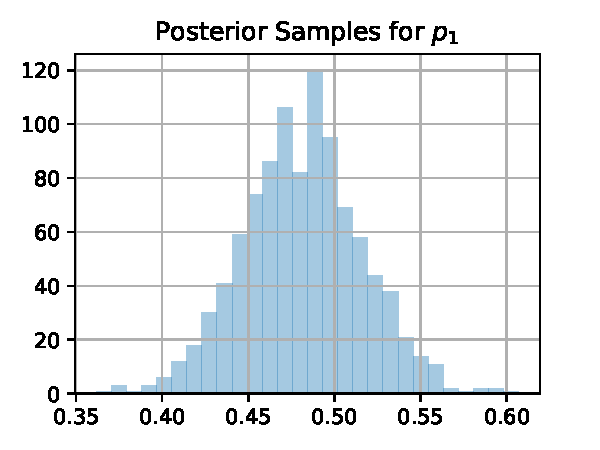
\includegraphics{p1_p1.pdf}
        \caption{1,000 samples from the posterior $p_1 \mid x_1$.}
        \label{fig:p1_p1_dist}
      \end{figure}

      \begin{figure}        
        \centering
        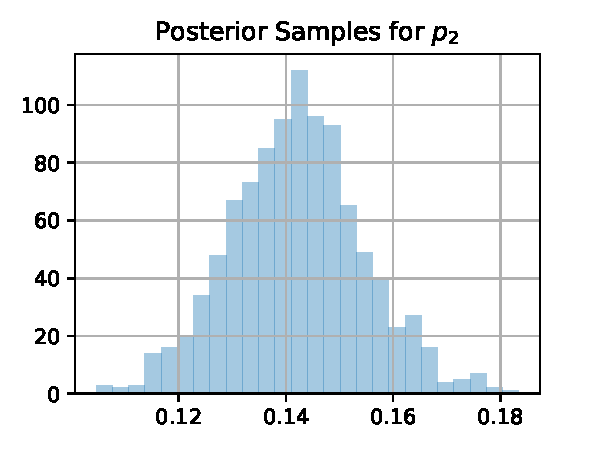
\includegraphics{p1_p2.pdf}
        \caption{1,000 samples from the posterior $p_2 \mid x_2$.}
        \label{fig:p1_p2_dist}
      \end{figure}

      The sample 90\% interval for $p_1$ was $(0.4255, 0.5393)$. The sampled
      90\% intervals for $p_2$ were $(0.1209, 0.1634)$, which agree with the
      previous interval calculations.
    \end{description}
  \item Obtain samples from the posterior distribution of $\theta | x_1,x_2$ and
    form the histogram representation of the posterior. Obtain the posterior
    median and 90\% credible interval for $\theta \mid x_1, x_2$ and compare
    with the likelihood analysis.
    \begin{description}
    \item[Solution:] To get a posterior sample for $\theta$, we draw samples
      from $p_1 \mid x_1$ and $p_2 \mid x_2$ and calculate $\theta$. The samples
      can be seen in Figure \ref{fig:p1_theta_dist}.

      \begin{figure}        
        \centering
        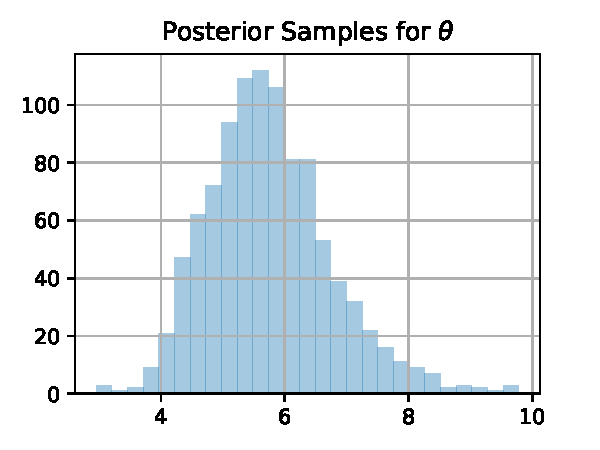
\includegraphics{p1_theta.pdf}
        \caption{1,000 samples from the posterior $\theta \mid x_2$.}
        \label{fig:p1_theta_dist}
      \end{figure}

      The samples 90\% credible interval was $(6.3137, 6.4755)$, and the sampled
      posterior median was $5.6486$. The median is very close to the MLE in
      Equation \ref{eqn:p1_theta_mle}. The 90\% credible interval is much
      smaller however since we make the prior beta assumption for $p_1$ and
      $p_2$.

      The computations for the analysis can be found in
      \href{https://nbviewer.jupyter.org/github/ppham27/stat570/blob/master/hw5/case\_control.ipynb}{\texttt{case\_control.ipynb}}.
    \end{description}    
  \item Suppose the rate of esophageal cancer is 18 in 100,000. Describe how
    this information may be used to evaluate
    $q_1 = \mathbb{P}\left(Y = 1 \mid X = 1\right)$ and
    $q_0 = \mathbb{P}\left(Y = 1 \mid X = 0\right)$.
    \begin{description}
    \item[Solution:] We can apply Bayes' rule since we know
      $\mathbb{P}\left(Y = 1\right) = 9/50,000 = 0.00018$ and
      $\mathbb{P}\left(Y = 0\right) = 49,991/50,000 = 0.99982$.

      Thus, we have that
      \begin{align*}
        \mathbb{P}\left(Y = 1 \mid X = 1\right)
        &= \frac{\mathbb{P}\left(X = 1 \mid Y = 1\right)\mathbb{P}\left(Y = 1\right)}
          {\mathbb{P}\left(X = 1 \mid Y = 0\right)\mathbb{P}\left(Y = 0\right) +
          \mathbb{P}\left(X = 1 \mid Y = 1\right)\mathbb{P}\left(Y = 1\right)} \\
        &= \frac{p_1\mathbb{P}\left(Y = 1\right)}
          {p_2\mathbb{P}\left(Y = 0\right) + p_1\mathbb{P}\left(Y = 1\right)} \\
        \mathbb{P}\left(Y = 1 \mid X = 0\right)
        &= \frac{\mathbb{P}\left(X = 0 \mid Y = 1\right)\mathbb{P}\left(Y = 1\right)}
          {\mathbb{P}\left(X = 0 \mid Y = 0\right)\mathbb{P}\left(Y = 0\right) +
          \mathbb{P}\left(X = 0 \mid Y = 1\right)\mathbb{P}\left(Y = 1\right)} \\
        &= \frac{\left(1 - p_1\right)\mathbb{P}\left(Y = 1\right)}
          {\left(1 - p_2 \right)\mathbb{P}\left(Y = 0\right) + \left(1 - p_1\right)\mathbb{P}\left(Y = 1\right)}.
      \end{align*}

      We can either substitute the the MLE $\hat{p}_i$ for $p_i$ or integrate
      over the posteriors $p_1 \mid x_1$ and $p_2 \mid x_2$.

      For example, the MLE estimates are $\hat{q}_1 \approx 0.0006140$ and
      $\hat{q}_2 \approx 0.0001089$.
    \end{description}
  \end{enumerate}
\item
  \begin{enumerate}
  \item Consider the likelihood,
    $\hat\theta \mid \theta \sim \mathcal{N}\left(\theta,V\right)$ and the prior
    $\theta \sim \mathcal{N}\left(0,W\right)$ with $V$ and $W$ known. Show that
    $\theta \mid \hat{\theta} \sim \mathcal{N}\left(r\hat{\theta},rV\right)$, where
    $r=W/\left(V +W\right)$.
    \begin{description}
    \item[Solution:] This result follows from the conjugacy of the normal
      distribution with itself:
      \begin{align}
        p\left(\theta \mid \hat{\theta}\right)
        &\propto p\left(\hat{\theta}\mid \theta \right)p\left(\theta\right) \nonumber\\
        &\propto \exp\left(
          -\frac{1}{2V}\left(\hat{\theta} - \theta\right)^2
          -\frac{1}{2W}\theta^2
          \right) \nonumber\\
        &\propto \exp\left(
          -\frac{V + W}{2\left(VW\right)}
          \left(\frac{W}{V+W}\hat{\theta}^2 -2\frac{W}{V+W}\hat\theta\theta + \theta^2\right)
          \right) \nonumber\\
        &\propto \exp\left(
          -\frac{V + W}{2\left(VW\right)}
          \left(\theta - \frac{W}{V+W}\hat{\theta}\right)^2
          \right) = \exp\left(
          -\frac{1}{2\left(rV\right)}
          \left(\theta - r\hat{\theta}\right)^2
          \right) \nonumber
      \end{align}
      after completing the square. We recognize this distribution as being part
      of the normal family, which gives us the result.
    \end{description}
  \item Suppose we wish to compare the models $M_0$: $\theta = 0$ versus $M_1$:
    $\theta \neq 0$. Show that the Bayes factor is given by
    \begin{equation}
      \frac{p\left(\hat\theta \mid M_0\right)}{p\left(\hat\theta \mid M_1\right)}
      = \frac{1}{\sqrt{1-r}}\exp\left(-\frac{Z^2}{2}r\right),
      \label{eqn:p2_bayes_factor}
    \end{equation}
    where $Z = \hat{\theta}/\sqrt{V}$.

    \begin{description}
    \item[Solution:] We have that
      \begin{align*}
        p\left(\hat{\theta} \mid M_0\right)
        &= p\left(\hat{\theta} \mid \theta = 0\right)
          = \frac{1}{\sqrt{2\pi V}}\exp\left(-\frac{1}{2V}\hat{\theta}^2\right) \\
        p\left(\hat{\theta} \mid M_1\right)
        &= \int_{-\infty}^\infty p\left(\hat{\theta} \mid \theta\right)p\left(\theta\right)\,\mathrm{d}\theta \\
        &= \frac{1}{\sqrt{2\pi\left(V + W\right)}}\exp\left(
          -\frac{1}{2\left(V + W\right)}\hat\theta^2
          \right)
      \end{align*}
      after completing the square. Substituting into the left-hand side of
      Equation \ref{eqn:p2_bayes_factor}, we obtain
      \begin{equation*}
        \frac{p\left(\hat\theta \mid M_0\right)}{p\left(\hat\theta \mid M_1\right)}
        = \sqrt{\frac{V+W}{V}}\exp\left(-\frac{1}{2}\cdot \frac{W}{V+W} \cdot \frac{\hat\theta^2}{V}\right)
        = \frac{1}{\sqrt{1-r}}\exp\left(-\frac{Z^2}{2}r\right)
      \end{equation*}
      as desired. 
    \end{description}
  \item Suppose we have a prior probability $\pi_1 = \mathbb{P}\left(M_1\right)$
    of model $M_1$ being true. Write down an expression for the posterior
    probability $\mathbb{P}\left(M_1 \mid \hat{\theta}\right)$ in terms of the
    Bayes factor.
    \begin{description}
    \item[Solution:] Let $K$ be the Bayes factor. By applying Bayes' rule, we
      have that
      \begin{align*}
        \mathbb{P}\left(
          M_1 \mid \hat\theta
        \right)
        &=
        \frac
        {\mathbb{P}\left(\hat\theta \mid M_1\right)\mathbb{P}\left(M_1\right)}
        {\mathbb{P}\left(\hat\theta \mid M_0\right)\mathbb{P}\left(M_0\right) +
          \mathbb{P}\left(\hat\theta \mid M_1\right)\mathbb{P}\left(M_1\right)} \\
        &= \frac
          {K^{-1}\mathbb{P}\left(\hat\theta \mid M_0\right)\pi_1}
        {\mathbb{P}\left(\hat\theta \mid M_0\right)\left(1 - \pi_1\right) +
          K^{-1}\mathbb{P}\left(\hat\theta \mid M_0\right)\pi_1} \\
        &= \frac
          {K^{-1}\pi_1}
          {\left(1 - \pi_1\right) + K^{-1}\pi_1}
          = \frac
          {\pi_1}{K\left(1 - \pi_1\right) + \pi_1}.
      \end{align*}
    \end{description}
  \item Now suppose we have summaries from two studies, $\theta_j$, $V_j$,
    $j = 1,2$. Assuming,
    $\theta_j \mid \theta \sim \mathcal{N}\left(\theta, V_j\right)$ and the
    prior $\theta \sim \mathcal{N}\left(0,W\right)$, derive the posterior
    $p\left(\theta \mid \theta_1,\theta_2\right)$.
    \begin{description}
    \item[Solution:] We have
      \begin{align*}
        p\left(\theta \mid \theta_1,\theta_2\right)
        &\propto
          p\left(\theta_2 \mid \theta_1, \theta \right)
          p\left(\theta_1 \mid \theta \right)p\left(\theta\right)
          =
          p\left(\theta_2 \mid \theta \right)
          p\left(\theta_1 \mid \theta \right)p\left(\theta\right) \\
        &\propto
          \exp\left(
          -\frac{1}{2V_2}
          \left(\theta_2 - \theta\right)^2
          \right)
          \exp\left(
          -\frac{V_1 + W}{2\left(V_1W\right)}
          \left(\theta - \frac{W}{V_1+W}\theta_1\right)^2
          \right) \\
        &\propto
          \exp\left(
          -\frac{V_1V_2 + V_1W + V_2W}{2\left(V_1V_2W\right)}
          \left(
          \theta - \frac{V_2W\theta_1 + V_1W\theta_2}{V_1V_2 + V_1W + V_2W}
          \right)^2
          \right),
      \end{align*}
      after repeatedly completing the square and dropping factors that don't
      depend on $\theta$.

      Thus, we have that
      \begin{equation}
        \theta \mid \theta_1,\theta_2 \sim \mathcal{N}\left(
          \frac{V_2W\theta_1 + V_1W\theta_2}{V_1V_2 + V_1W + V_2W},
          \frac{V_1V_2W}{V_1V_2 + V_1W + V_2W}
        \right).
      \end{equation}
    \end{description}
  \item Derive the Bayes factor
    \begin{equation}
      \frac{p\left(\theta_1,\theta_2\mid M_0\right)}
      {p\left(\theta_1,\theta_2\mid M_1\right)},
    \end{equation}
    again comparing the models $M_0$: $\theta = 0$ versus $M_1$:
    $\theta \neq 0$.

    \begin{description}
    \item[Solution:] $\left(\theta_1,\theta_2\right)$ have a bivariate normal
      distribution. Under $M_0$, we have that
      \begin{align}
        p\left(\theta_1,\theta_2 \mid M_0\right)
        &= p\left(\theta_1,\theta_2 \mid \theta = 0\right) \nonumber\\
        &= \frac{1}{2\pi\sqrt{V_1V_2}}\exp\left(
          -\frac{1}{2}
          \begin{pmatrix}
            \theta_1 & \theta_2
          \end{pmatrix}
                       \begin{pmatrix}
                         \frac{1}{V_1} & 0 \\
                         0 & \frac{1}{V_2}
                       \end{pmatrix}
                       \begin{pmatrix}
                         \theta_1 \\ \theta_2
                       \end{pmatrix}
          \right).
      \end{align}
      
      Under $M_1$, we have that
      \begin{align}
        p\left(\theta_1,\theta_2 \mid M_1\right)
        &= \int_{-\infty}^\infty p\left(\theta_1,\theta_2 \mid \theta\right)
          p\left(\theta\right)\,\mathrm{d}\theta.
      \end{align}
      We can consider $\theta$ as having the improper prior
      $\mathcal{N}\left(\mathbf{0}, \begin{pmatrix} W & W \\ W &
          W \end{pmatrix}\right),$ which results in
      \begin{equation}
        \theta_1,\theta_2 \mid M_1 \sim \mathcal{N}\left(
          \mathbf{0}, \begin{pmatrix}
            V_1 + W & W \\
            W & V_2 + W
          \end{pmatrix}          
        \right)
      \end{equation}
      by conjugacy of the multivariate normal distribution.

      The Bayes factor can then be computed:
      \begin{equation}
        \sqrt{\frac{V_1V_2 + V_1W + V_2W}{V_1V_2}}
        \exp\left(
          -\frac{1}{2}
          \begin{pmatrix}
            \theta_1 & \theta_2
          \end{pmatrix}
          \Lambda
          \begin{pmatrix}
            \theta_1 \\ \theta_2
          \end{pmatrix}
        \right),
      \end{equation}
      where \begin{equation}
        \Lambda =
        \begin{pmatrix}
          \frac{1}{V_1} & 0 \\
          0 & \frac{1}{V_2}
        \end{pmatrix}
        + \frac{1}{V_1V_2 + V_1W + V_2W}
        \begin{pmatrix}
          V_2 + W & -W \\
          -W & V_1 + W
        \end{pmatrix}.
      \end{equation}
    \end{description}
  \item We will show these results can be used in the context of a genome-wide
    association study on Type II diabetes, reported by Frayling et al. (2007,
    Science). Two sets of data were independently collected, resulting in two
    log odds ratios $\hat{\theta}_j$, $j = 1,2$, for each SNP.
     
    For SNP rs9939609 point estimates (95\% confidence intervals) were 1.27
    (1.16, 1.37) and 1.15 (1.09,1.23). Suppose we have a normal prior for the
    odds ratio that has a 95\% range (0.67, 1.50).

    \begin{enumerate}
    \item Find W from this interval, and then calculate the posterior median and
      95\% intervals for $\theta$ based on (i) the first dataset only, (ii) both
      of the populations.
      \begin{description}
      \item[Solution:] The analysis can be found at
        \href{https://nbviewer.jupyter.org/github/ppham27/stat570/blob/master/hw5/genome\_association.ipynb}{\texttt{genome\_association.ipynb}}.
      \end{description}
      
    \item 
    \item 
    \end{enumerate}
  \end{enumerate}
\item We will carry out a Bayesian analysis of the lung cancer and radon data,
  that were examined in lectures, using INLA. These data are available on the
  class website. The likelihood is
  $Y_i \mid \beta \sim \operatorname{Poisson}\left (E_i\exp\left(\beta_0 +
      \beta_1x_i\right)\right)$ independently distributed, where
  $\beta = \begin{pmatrix}\beta_0 & \beta_1\end{pmatrix}^\intercal$, $Y_i$ and
  $E_i$ are observed and expected counts of lung cancer incidence in Minnesota
  in 1998--2002, and $x_i$ is a measure of residential radon in county $i$,
  $i = 1,\ldots,n$.

  \begin{enumerate}
  \item Analyze these data using the default prior specifications in
    INLA. Produce figures of the INLA approximations to the marginal
    distributions of $\beta_0$ and $\beta_1$, along with the posterior means,
    posterior standard deviations, and 2.5\%, 50\%, 97.5\% quantiles.

    \begin{description}
    \item[Solution:]
      \begin{figure}
        \centering
        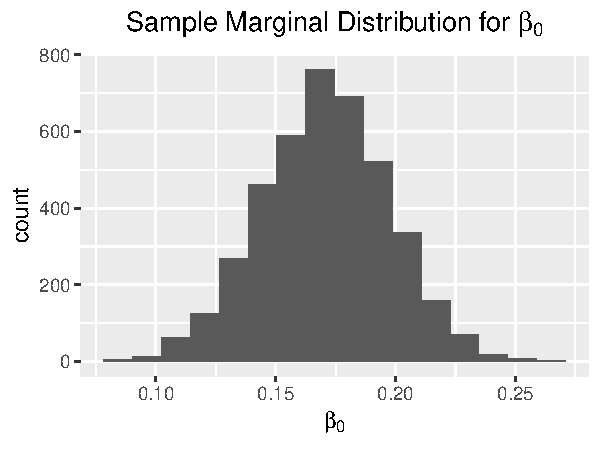
\includegraphics{p3_beta_0.pdf}
      \end{figure}

      \begin{figure}
        \centering
        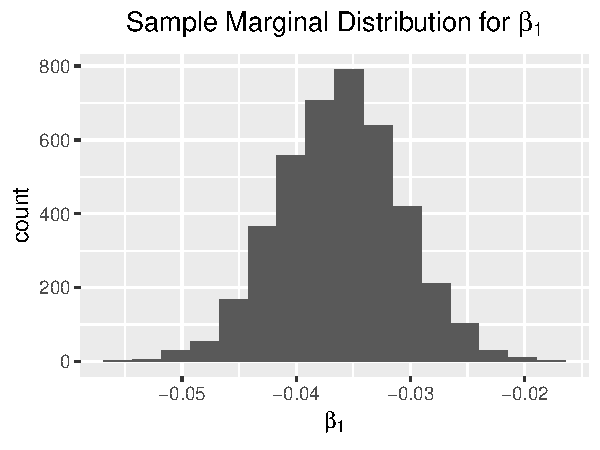
\includegraphics{p3_beta_1.pdf}
      \end{figure}

      \begin{figure}
        \centering
        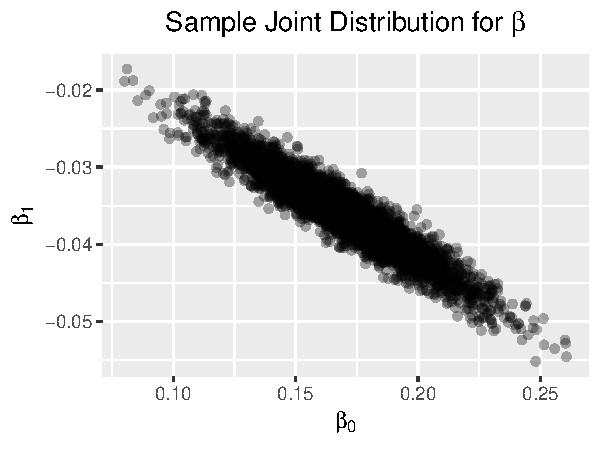
\includegraphics{p3_beta_joint.pdf}
      \end{figure}
      
      Details of the analysis can be found in
      \href{https://nbviewer.jupyter.org/github/ppham27/stat570/blob/master/hw5/lung\_cancer\_radon.ipynb}{\texttt{lung\_cancer\_radon.ipynb}}.
    \end{description}
  \item For a more informative prior specification we may reparameterize the
    model as independently distributed
    \begin{equation}
      Y_i \mid \theta \sim \operatorname{Poisson}\left(
        E_i\theta_0\theta_1^{x_i - \bar{x}_i}
      \right),
    \end{equation}
    where
    $\theta = \begin{pmatrix} \theta_0 & \theta_1\end{pmatrix}^\intercal$ and
    \begin{equation}
      \theta_0 = \mathbb{E}\left[\frac{Y}{E} \mid x = \bar{x}\right]
      = \exp\left(\beta_0 + \beta_1\bar{x}\right)
    \end{equation}
    where is the expected standardized mortality ratio in an area with average
    radon. The parameter $\theta_1 = \exp\left(\beta_1\right)$ is the relative
    risk associated with a one-unit increase in radon.  For $\theta_0$ we assume
    a lognormal prior with 2.5\% and 97.5\% quantiles of 0.67 and 1.5 to give
    $\mu = 0$ and $\sigma = 0.21$. For $\theta_1$ we again take a lognormal
    prior and assume the relative risk associated with a one-unit increase in
    radon is between 0.8 and 1.2 with probability 0.95, to give $\mu = -0.02$
    and $\sigma = 0.10$. By converting these into normal priors in INLA, rerun
    your analysis, and report the same summaries.

    \begin{description}
    \item[Solution:] For the priors, we have two independent normals
      \begin{align*}
        \log\theta_0
        &\sim \mathcal{N}\left(0, 0.21^2\right) \\
        \log\theta_1
        &\sim \mathcal{N}\left(-0.02, 0.1^2\right).
      \end{align*}

      We can rewrite
      \begin{equation}
        E_i\theta_0\theta_1^{x_i - \bar{x}_i} = E_i\exp\left(
          \log\theta_0 + \left(x_i - \bar{x}\right)\log\theta_1
        \right),
      \end{equation}
      so after centering the $x_i$, we can specify priors on the intercept and
      coefficients as usual.
    \end{description}
  \end{enumerate}
\item Consider the simple linear regression model
  $Y_i = \beta_0 + \beta_1x_i + \epsilon_i$, with
  $\epsilon_i \mid \sigma^2 \sim_\mathrm{iid} \mathcal{N}\left(0,
    \sigma^2\right)$, $i = 1,\ldots, n$. Suppose the prior distribution is of the
  form
  \begin{equation}
    \pi\left(\beta_0,\beta_1,\sigma^2\right) = \pi\left(\beta_0,\beta_1\right)
    \pi\left(\sigma^{-2}\right).
  \end{equation}

  The prior for $\begin{pmatrix}\beta_0 & \beta_1\end{pmatrix}^\intercal$ is
  \begin{equation}
    \begin{pmatrix}
      \beta_0 \\ \beta_1
    \end{pmatrix} \sim
    \mathcal{N}\left(
      \begin{pmatrix}
        m_0 \\ m_1
      \end{pmatrix},
      \begin{pmatrix}
        v_{00} & v_{01} \\ v_{01} & v_{11}
      \end{pmatrix} 
    \right)
  \end{equation}
  and the prior for $\sigma^{-2}$ is $\operatorname{Gamma}\left(a, b\right)$. In
  this exercise the conditional distribution required for Gibbs sampling will be
  derived.

  \begin{enumerate}
  \item Write down the form of the posterior distribution (up to
    proportionality) and derive the conditional distributions
    $p\left(\beta_0 \mid \beta_1, \sigma^2, \mathbf{y}\right)$,
    $p\left(\beta_1 \mid \beta_0, \sigma^2, \mathbf{y}\right)$ and
    $p\left(\sigma^2 \mid \beta_0, \beta_1, \mathbf{y}\right)$. Hence, give details of the
    Gibbs sampling algorithm.

    \begin{description}
    \item[Solution:] Using the normal likelihood and prior, we have the posterior
      \begin{align*}
        p\left(\beta_0, \beta_1, \sigma^2\mid \mathbf{y}\right)
        &\propto p\left(\mathbf{y} \mid \beta_0, \beta_1, \sigma^2\right)\pi\left(
          \beta_0,\beta_1,\sigma^2
          \right) \\
        &\propto
          \pi\left(\beta_0,\beta_1\right)
          \pi\left(\sigma^{-2}\right)
          \left(\frac{\sigma^{-2}}{2\pi}\right)^{n/2}
          \prod_{i=1}^n
          \exp\left(
          -\frac{1}{2\sigma^2}\left(y_i - \beta_0 + \beta_1x_i\right)^2
          \right),
      \end{align*}
      where
      \begin{align*}
        \pi\left(\beta_0,\beta_1\right)
        &\propto \exp\left(-\frac{1}{2}
        \left(\beta - m\right)^\intercal V^{-1}\left(\beta - m\right)
        \right),~\text{where}~V=\begin{pmatrix}
        v_{00} & v_{01} \\ v_{01} & v_{11}
      \end{pmatrix} \\
        \pi\left(\sigma^{-2}\right)
        &\propto
        \left(\sigma^{-2}\right)^{a-1}\exp\left(-b\sigma^{-2}\right).
      \end{align*}

      For $p\left(\sigma^2 \mid \beta_0, \beta_1, \mathbf{y}\right)$, we can
      drop all the factors without $\sigma^2$, so we have
      \begin{align*}
        p\left(\sigma^2 \mid \beta_0, \beta_1, \mathbf{y}\right)
        &\propto
          \left(\sigma^{-2}\right)^{a + n/2 -1}\exp\left(-b\sigma^{-2}\right)
          \prod_{i=1}^n
          \exp\left(
          -\frac{1}{2\sigma^2}\left(y_i - \beta_0 + \beta_1x_i\right)^2
          \right) \\
        &\propto
          \left(\sigma^{-2}\right)^{a + n/2 -1}\exp\left(
          -\sigma^{-2}\left(b + \frac{1}{2}\sum_{i=1}^n\left(y_i - \beta_0 - \beta_1x_i\right)^2\right)
          \right),
      \end{align*}
      so $\boxed{\left(\sigma^{-2} \mid \beta_0, \beta_1, \mathbf{y} \right)\sim \operatorname{Gamma}\left(
          a + \frac{n}{2}, b + \frac{1}{2}\sum_{i=1}^n\left(y_i - \beta_0 - \beta_1x_i\right)^2\right).}$

      
      The conditional posteriors for $\beta_0$ and $\beta_1$ can be obtained
      from marginalizing $p\left(\beta \mid \sigma^2, \mathbf{y}\right)$ from
      the next part. We'll get
      \begin{align*}
        \left(\beta_0 \mid \beta_1, \sigma^2, \mathbf{y}\right)
        &\sim \mathcal{N}\left(m^*_1, V^*_{11}\right) \\
        \left(\beta_1 \mid \beta_0, \sigma^2, \mathbf{y}\right)
        &\sim \mathcal{N}\left(m^*_2, V^*_{22}\right).
      \end{align*}
    \end{description}
  \item Another blocked Gibbs sampling algorithm would simulate from the
    distributions $p\left(\beta \mid \sigma^2, \mathbf{y}\right)$ and
    $p\left(σ^{-2} \mid \beta, \mathbf{y}\right)$. Derive the distributions
    \begin{align}
      \left(\beta \mid \sigma^2, \mathbf{y} \right)
      &\sim \mathcal{N}\left(m^*, V^*\right)
      \label{eqn:p4_beta_posterior} \\
      \left(\sigma^2 \mid \beta, \mathbf{y} \right)
      &\sim \operatorname{Gamma}\left(
      a + \frac{n}{2}, b + \frac{1}{2}\left(\mathbf{y} - X\beta\right)^\intercal
      \left(\mathbf{y} - X\beta\right)
      \right),
      \label{eqn:p4_sigma_posterior}
    \end{align}
    where
    \begin{align*}
      m^* &= W\hat{\beta} + \left(I_2 - W\right)m \\
      V^* &= W\operatorname{Var}\left(\hat{\beta}\right)
    \end{align*}
    and $W = \left(X^\intercal X + V^{-1}\sigma^2\right)^{-1}X^\intercal X$ and
    $\hat{\beta}$ is the MLE of $\beta$.

    \begin{description}
    \item[Solution:] Let $X$ be the a $n \times 2$ matrix with all $1$s in the
      first column and $\begin{pmatrix} x_1 \cdots x_n\end{pmatrix}^\intercal$
      as the second column.

      Then, Equation \ref{eqn:p4_sigma_posterior} follows from the previous part
      after rewriting the term
      \begin{equation}
        \frac{1}{2}\sum_{i=1}^n\left(y_i - \beta_0 - \beta_1x_i\right)^2
        = \frac{1}{2}\left(\mathbf{y} - X\beta\right)^\intercal\left(\mathbf{y} - X\beta\right).
      \end{equation}

      As before, we complete the square to derive the posterior for $\beta$:
      \begin{align*}
        &\left(\mathbf{y} - X\beta\right)^\intercal \sigma^{-2}I_n\left(\mathbf{y} - X\beta\right)
        + \left(\beta - m\right)^\intercal V^{-1}\left(\beta - m\right) \\
        &= \beta^\intercal \sigma^{-2}X^\intercal X \beta + \beta^\intercal V^{-1} \beta
          - 2\beta^\intercal\left(\sigma^{-2}X^\intercal y + V^{-1}m\right) +
          \sigma^{-2}y^\intercal y - m^\intercal V^{-1}m \\
        &= \beta^\intercal\left(
          \sigma^{-2}X^\intercal X + V^{-1}
          \right)\beta \\
        &~~~
          -2 \beta^\intercal          
          \left(
          \sigma^{-2}X^\intercal X + V^{-1}
          \right)
          \left(
          \sigma^{-2}X^\intercal X + V^{-1}
          \right)^{-1}
          \left(\sigma^{-2}X^\intercal y + V^{-1}m\right) + C,
      \end{align*}
      where we have collapsed the terms that don't depend on $\beta$ into $C$.

      Recall that
      $\operatorname{Var}\left(\hat{\beta}\right) = \sigma^2\left(X^\intercal
        X\right)^{-1}$, so we have that
      \begin{equation*}
        \left(\sigma^{-2}X^\intercal X + V^{-1}\right)^{-1}
        = \left(X^\intercal X + \sigma^{2}V^{-1}\right)^{-1}\left(X^\intercal X\right)
        \sigma^2\left(X^\intercal X\right)^{-1} = V^*,
      \end{equation*}
      so continuing the process of completing the square:
      \begin{align*}
        &\beta^\intercal\left(V^*\right)^{-1}\beta -
          2\beta^\intercal\left(V^*\right)^{-1}
          W\left(X^\intercal X\right)^{-1}\left(X^\intercal y + \sigma^2 V^{-1}m\right) + C \\
        &= \beta^\intercal\left(V^*\right)^{-1}\beta -
          2\beta^\intercal\left(V^*\right)^{-1}\left(
          W\hat\beta + W\sigma^2\left(X^\intercal X\right)^{-1}V^{-1}m
          \right) + C \\
        &= \beta^\intercal\left(V^*\right)^{-1}\beta
          - 2\beta^\intercal\left(V^*\right)^{-1}\left(
          W\hat\beta + \sigma^2\left(V\left(X^\intercal X + \sigma^2V^{-1}\right)\right)^{-1}m
          \right) + C \\
        &= \beta^\intercal\left(V^*\right)^{-1}\beta
          - 2\beta^\intercal\left(V^*\right)^{-1}\left(
          W\hat\beta + \sigma^2\left(VX^\intercal X + \sigma^2I\right)^{-1}m
          \right) + C \\
        &= \beta^\intercal\left(V^*\right)^{-1}\beta
          - 2\beta^\intercal\left(V^*\right)^{-1}\left(
          W\hat\beta + \left(I_2 - W\right)m\right) + C \\
        &= \left(\beta - m^*\right)^\intercal \left(V^*\right)^{-1}\left(\beta - m^*\right)
           + C^\prime,
      \end{align*}
      where we have applied the
      \href{https://en.wikipedia.org/wiki/Woodbury\_matrix\_identity}{Woodbury
        matrix identity}.

      Thus, all the factors that contain $\beta$ can be written as a quadratic
      form which gives us the result in Equation \ref{eqn:p4_beta_posterior}.
    \end{description}
  \end{enumerate}
  
\end{enumerate}
\end{document}
